
\chapter{Theory: basic relaxation methods}  %Title of the First Chapter
\label{chap.basic}

This chapter offers an overview of the core relaxation methods utilized in this thesis. While there is a wide variety of MINLP problem types, there are established relaxation tools readily available in the existing literature. Consequently, when tackling a MINLP problem, one can explore these readily accessible tools and select the most appropriate one to meet their specific requirements. These relaxation tools can be categorized as follows: relaxations via lifting, relaxations via submodularity, relaxations via piece-wise linear functions, and relaxations tightening via intersection cuts.

\section{Relaxations via lifting}


In this section, we present a meta-relaxation method known as  ``lifting''. Lifting involves the approximation of a set by representing it in a higher-dimensional space, thereby providing greater flexibility in addressing challenging problems. In this section, we present several lifting-based relaxation methods: Dantzig-Wolfe relaxations, factorable programming relaxations, and certificate-based relaxations. We also present the projection method that can project a high-dimensional sets into a lower dimensional space.

We have established that any MINLP problem can be reformulated into a linear optimization problem over its feasible set, which may be nonconvex. The MINLP problem's feasible set is denoted as $K \in \mathbb{R}^n$, and we approach the MINLP problem in the form of $\min_{x \in K} cx$. To construct the extended formulation of the MINLP problem, we adopt a set-theoretic approach that relies on representing the nonconvex set $K$ in a higher-dimensional space through lifting.

\begin{definition}
    For the nonconvex set $K \in \bR^n$, its convex hull admits a lifted representation $K' \in \bR^{n+k}$ for $k \ge 1$, if $\conv(K)= \proj_{\bR^n}(K')$.
\end{definition}

In some cases, lifting simplifies the process of constructing the convex hull for the nonconvex feasible set $K$. Let $c' = (c,0)$ where $0 \in \bR^k$. We have the following equalities:

\begin{equation}
    \min_{x \in K} cx  = \min_{x \in \conv(K)} cx = \min_{y \in K'} c'y.
\end{equation}

As $y$ is in the extended space containing $x$, we refer to $\min_{y \in K'} c'y$ as an extended formulation of the MINLP problem. In situations where constructing $K'$ is not feasible, we instead search for a convex set $\bar{K'}$ that includes $K'$. The convex outer approximation $\bar{K'}$ remains valuable as it provides a relaxation $\min_{y \in \bar{K'}} c'y$ in the extended space. We term this relaxation an \emph{extended relaxation}, which satisfies that
\begin{equation}
    \min_{y \in K'} c'y \ge \min_{y \in \bar{K'}} c'y.
\end{equation}

The lifting method offers extended formulations or extended relaxations for the MINLP problem. We have the option to solve the extended formulations/relaxations directly or improve the original projected formulations/relaxations by incorporating the results from lifting.



\subsection{Dantzig-Wolfe relaxation}
\label{chap.sec.dwrel}
The first lifting method utilizes a geometric approach based on Dantzig-Wolfe (DW) relaxation \cite{gilmore1961linear,Vanderbeck2010}, which proves to be widely applicable whenever all extreme points of a nonconvex set can be enumerated. The method of the DW relaxation involves an implicit generation of convex combination of those extreme points, and, in some cases, to obtain a relaxation, the method may not exhaust all the extreme points.

Consider $K = K_1 \cap K_2$. We assume that computing the convex hulls of both $K_1$ and $K_2$ is straightforward, and we also have a lifted representation, denoted as $K'_2$, such that $\conv(K_2) = \proj_{\bR^n}(K'_2)$. With these assumptions in place, we can derive a convex outer approximation $\bar{K}$ using the following procedure.

\begin{lemma}
\label{lem.dw}
    $K \subseteq \bar{K} :=\conv(K_1) \cap  \proj_{\bR^n}(K'_2)$.
\end{lemma}
\begin{proof}
    The convex hull of the intersection of two sets is included in the intersection of the convex hulls of the two sets.
\end{proof}


In the following, we consider exclusively the sets with  polytope convex hulls, for which one can generate all their extreme points in a finite time. It is noteworthy that a convex set may have an infinite number of extreme points, and we could in principle extend our methods for such case.

It is important to note that a polytope can have two different representations: the hyperplane representation and the vertex representation. In the case where $\conv(K_2)$ is a polytope and its vertices $V_2$ are known, we can examine its vertex representation. An explicit lifted representation of $\conv(K_2)$ can be defined as follows:
\begin{equation}
    K'_2 = \{(x,y) \in \bR^n \times \bR^{V_2}_+: \sum_{v \in V_2} y_v = 1 \land \ x = \sum_{v \in V_2}  y_v v\},
\end{equation}
where $k = |V_2|$. We note that $\conv(K_2) = \conv(V_2) = \proj_{\bR^n}(K'_2)$. 


By \Cref{lem.dw}, the problem $\min_{x \in \bar{K}} cx$ is a convex relaxation of $\min_{x \in K} cx$. As  $ \bar{K} =\conv(K_1) \cap  \proj_{\bR^n}(K'_2)$, we call the relaxation \emph{DW relaxation}. In addition, the DW relaxation admits the following simplified form:
 \begin{subequations}
    \label{dwrel}
    \begin{align}
       \dw(V):=\min &  \quad c \sum_{v \in V}  y_v v  \\
    \mst &  \quad  \sum_{v \in V}  y_v v  \in \conv(K_1) \\
       &  \quad  \sum_{v \in V} y_v = 1\\
      & \quad y \in \bR^{V}_+,
    \end{align}
\end{subequations}
where $V = V_2$ and $x$ is substituted by $\sum_{v \in V_2}  y_v v$. 
However, the number of vertices $V_2$ can be exponential in $n$, and this limits the tractability  of the DW relaxation. 


The column generation method \cite{barnhart1998branch,Vanderbeck2010} is employed to address this issue. It begins by considering a subset $V'_2$ of the vertices $V_2$ and then solves the restricted problem $\dw(V'_2)$. Next, it searches for a point (column) $v \in V_2 \setminus V'_2$ that can improve the restricted problem and adds this column to $V'_2$. This process iterates, resulting in a sequence of non-increasing upper bounds $\dw(V'_2)$. Finally, the column generation process stops generating new columns once the bound converges, \ie $\dw(V_2) = \dw(V'_2)$.


The column generation process should determine whether and how to generate a column. We assume that $\conv(K_1)$ is a polytope with a known hyperplane representation, \ie $\conv(K_1)=\{x \in \bR^n: \forall i \in [m], a^ix \le b_i\}$, where $a_i \in \bR^n, b_i \in \bR$. Consequently, the DW relaxation can be expressed as an LP:
 \begin{subequations}
    \label{dwrellp}
    \begin{align}
       \dw(V):=\min &  \quad c \sum_{v \in V}  y_v v  \\
    \mst \, \forall i \in [m] & \quad  a^i \sum_{v \in V}  y_v v  \le b_i \\
       &  \quad  \sum_{v \in V} y_v = 1\\
      & \quad y \in \bR^V_+.
    \end{align}
\end{subequations}

Since the strong duality  holds for LP, $\dw(V)$ equals the dual optimal value of the dual LP:
 \begin{subequations}
    \label{dwrelduallp}
    \begin{align}
       \dw(V):=\max  &  \quad  \lambda -\sum_{i \in [m]}  b_i \mu_i  \\
    \mst \; \forall v \in V & \quad \sum_{i \in [m]}a^i v  \mu_i + c v - \lambda \le 0 \\
       &  \quad  \mu \in \bR^m_+, \lambda \in \bR.
    \end{align}
\end{subequations}

The duality gives rise to  a certificate for the optimality of $\dw(V'_2)$ and a  verifiable condition to decide whether to generate a column. 

\begin{lemma}
  Let $\mu',\lambda'$ be the dual optimal solution to the dual problem for  $\dw(V'_2)$. If for all $v \in V_2 \setminus V'_2$,  $\sum_{i \in [m]}a^i v  \mu
  _i + c v - \lambda' \le 0$, then  $\mu'$ is also a dual optimal solution to the dual problem for  $\dw(V_2)$. 
\end{lemma}
\begin{proof}
    This condition implies that the dual solution is also feasible for the dual problem associated with $\dw(V_2)$, as the primal problem is already feasible. Thus, the primal value equals the dual value.  By the strong duality of LP, the primal-dual pairs are both optimal.
\end{proof}



Hence, if every constraint in $V_2$ is met by $\mu'$, then $\dw(V_2)$ equals $\dw(V'_2)$. At this point, the column generation process can be halted, and we can obtain the primal solution for $\dw(V'_2)$, which concurrently serves as a primal optimal solution for $\dw(V_2)$. To verify the  ``all-satisfied'' condition, it is sufficient to solve the following \emph{pricing subproblem}:

\begin{equation}
\label{eq.price}
    \max_{v \in V} \sum_{i \in [m]} a^i    \mu'_i v  + c v 
\end{equation}
and compare the maximum with $\lambda'$. If the maximum value of the pricing subproblem is strictly less than $\lambda'$, then the corresponding maximum argument is added to $V'_2$.  However, if the maximum value is equal to or greater than $\lambda'$,  it indicates that the primal and dual problems have converged, and the DW relaxation is considered solved.

We next consider a more concrete case, where $V = \{0,1\}^n \cap P$, and $P$ is a polytope given in hyper-plane representation. The pricing subproblem thus admits the following MILP representation:
\begin{equation}
\label{eq.priceref}
    \max_{x \in  P \cap \{0,1\}^n} (\sum_{i \in [m]} a^i    \mu'_i) x  + c x, 
\end{equation}
which can be solved by a MILP solver. In a more general setting, $P$ can be a convex set instead of a polyhedron.

\subsection{Projection}
A topic closely related to extended formulations is projections. In some cases, an explicit formulation of $\conv(K)$ is only known in the extended space, but it is more efficient and convenient to work in the original projected space.  The \emph{projection approach} seeks a low-dimensional approximation of $\proj_{\bR^n}(K')$.

In the following two cases, it becomes impractical to store the complete descriptions of $\conv(K)$ or $K'$.
Firstly, when given  $K'$ as a polytope,  the number of facets of $\proj_{\bR^n}(K')$ may be exponential in that of $K'$.  Secondly, if $K'$ is in vertex representation as $K'_2$, the number of auxiliary variables $y$ in its lifted representation can become very large. Consequently, this further hinders the storage of the entire representation.

To address these practical challenges, a cutting plane algorithm is used to iteratively refine a convex outer approximation of $K$ through projections. The algorithm operates like the column generation method for the dual LP.

Let us illustrate the usage of projection with an example. Vertex polyhedrality is a useful property for convexifying nonconvex functions in MINLP. A specific case is when a function is convex-extensible from vertices.
\begin{definition}
  Let $X$ be a polytope, and let $Q$ be the vertices of $X$. A function $f:X \to \bR$ is convex-extensible from vertices,  if
  \begin{multline}
    \conv({(x,t) \in X \times \bR: f(x) \le t}) =\\  \{(x,t) \in \bR^n \times \bR: \exists y \in  \bR^{Q}_+ \; \sum_{q \in Q} y_q = 1,  x = \sum_{q \in Q}  y_q q,  \sum_{q \in Q}  y_q f(q) \le t\}.
  \end{multline}
\end{definition}

A convex function $g $ is a \textit{convex underestimating function} of $f$ over $X$, if for all $x \in X$, $g(x) \le f(x)$.
The \textit{convex envelope} $\sF_f$ is defined as the maximal convex underestimating function of $f$ over $X$.
Hence, the convex envelope $\sF_{f}$ of a convex-extensible function $f$ is entirely determined by its values at vertices $Q$. The epigraph $K'$ of the convex envelope $\sF_{f}$ possesses a lifted representation that is similar to that of $K'_2$:
\begin{equation}
    K':= \{(x,y,t) \in \bR^n \times \bR^{Q}_+ \times \bR: \sum_{q \in Q} y_q = 1, x = \sum_{q \in Q}  y_q q,  \sum_{q \in Q}  y_q f(q) \le t\}.
\end{equation}

Let $(\tilde{x}, \tilde{t})$ be a point to be separated, where we can let $\tilde{t}$ be $f(\tilde{x})$ or other values.
The projection problem asks  a cutting plane $(a,1)$ to separate $(\tilde{x}, \tilde{t})$ from $\proj_{\bR^{n+1}}(K')$.  This separation problem can be formulated as the following LP:
 \begin{subequations}
    \label{seplp}
    \begin{align}
       \max &  \quad  a \tilde{x} +  \tilde{t}  \\
    \mst \,   \forall q \in Q & \quad aq +  f(q) \le 0\\
       &  \quad  (a,1) \in C,
    \end{align}
\end{subequations}
where $C$ is a convex set imposing the  boundedness of $(a,1)$.  In practice, $C$ is defined by a bound constraint on $L_1$ or $L_2$ norm of $(a,1)$, which is LP representable. A successful separation returns $(a,1)$ such that $a \tilde{x} +  \tilde{t} > 0$.

\begin{lemma}[\cite{falk1976successive}]
\label{thm.poly}
    Every concave function is convex-extensible from vertices.
\end{lemma}
Concave functions are not as tractable as convex functions, however, we can construct the convex envelopes of concave functions using the above results.


\subsection{Factorable programming}

We next present a second relaxation  approach that is widely adopted by MINLP optimization solvers. This approach relies on the symbolic representation of a mathematical program. The syntax and semantics of the symbolic representation can be defined formally. For brevity, we here only give a high-level introduction, and we refer to \cite{leoinbook,leonelson} for more details.


General nonconvex NLP problems typically admit the following  formulation:
 \begin{equation}
\label{minlp2}
	\min_{x \in \bR^n} \;  c\cdot x  \quad \suc \quad  Ax +  B g(x)\le d,
\end{equation}
where $c \in \bR^n, A \in \bR^{m \times n},  B \in \bR^{m \times k}, g: \bR^n \to \bR^k,  d \in \bR^m$. The map $g(x)$ represents a vector $(g_1(x),\dots,g_k(x))$ of nonconvex functions on $x$, and we refer to $g_i$  as its \emph{terms}. This formulation can be converted from the formulation \eqref{minlpref} through epigraphical reformulation.


The backend convex relaxation algorithms implemented in many general-purpose  solvers, including \baron, \couenne,  and \scip, are convex relaxations. Most of them further convert the convex relaxations into LP relaxations. These solvers leverage the separability present in the rows of $Ax+Bg(x)$, allowing them to relax and linearize  nonlinear terms $g_i$ individually. 



In the solvers' data structures, the problem \eqref{minlp2} is transformed into an extended formulation:
 \begin{equation}
 \label{minlp3}
	\min_{ (x,y) \in \bR^{n+k}} \;  c\cdot x  \quad \suc \quad  Ax +  B y\le d \; \land \; y = g(x).
\end{equation}
All the nonlinear terms are grouped within the nonconvex constraints $y = g(x)$. These constraints give rise to a nonconvex \emph{lifted set} defined as:
\begin{equation}
\label{eq.lift}
 \cSl \deq \{(x,y) \in \bR^{n+k}: y = g(x)\}.	 
\end{equation} 
In fact, one may find the above lifted structure similar to the DW relaxation. 
 
  
The relaxation algorithms employed by these solvers are based on factorable programming \cite{leoinbook, mccormick1976computability}: this approach treats the multivariate nonlinear terms $g_i$ as composite functions. These  algorithms commonly factor each $g_i$ into sums and products of a collection of univariate functions. If convex and concave relaxations of those univariate functions are available, these algorithms can linearize these relaxations, and yield a linear relaxation for Eq.~\eqref{minlp2}. Common lists of such univariate functions, that are usually available to all sBB solvers, include $t^a$ (for $a\in\mathbb{N}$), $\frac{1}{t}$, $\log{t}$, $\exp{t}$. Some solvers also offer a choice of trigonometric functions, e.g.~\couenne.  In this way, one can obtain a convex outer approximation of $\cSl$, which yields a convex relaxation of the NLP.


\subsection{Certificate-based relaxation}

The third lifting method is an algebraic method based on non-negativity certificates, and we call the relaxations derived from this method. It proves to be particularly useful for polynomial programming (PP) and related problems. An advantage of this method is that it does not necessitate box constraints, which are essential for many conventional relaxation methods. This relaxation method is based on the duality point of view.

Assume that we aim to solve the following problem:
\begin{equation}
\label{cerprim}
  \lambda^\ast :=  \min_{x \in K} f(x),
\end{equation}
where $K$ represents a complicated domain of the nonlinear function $f$. The problem has an equivalent dual formulation, which  searches for the maximum $\lambda \in \bR$ such that $f(x) -\lambda$ is non-negative over $K$:
\begin{equation}
\label{cerdual}
  \lambda^\ast:=  \max \{\lambda\in \bR: \forall x \in K\; f(x) - \lambda \ge 0\},
\end{equation}


We assume that $f_\lambda(x) := f(x) - \lambda$  belongs to a set $F$ of functions, such as polynomials. Let $F^{+}_{K}$ denote the set of non-negative functions in $F$ over $K$. Each function in $F^{+}_{K}$ is referred to as a \emph{non-negativity certificate}. Additionally, we assume that $F^{+}_{K}$ forms a convex cone, such as the cone of nonnegative polynomials. As a result, the dual problem \eqref{cerdual} becomes a convex optimization problem:
\begin{equation}
\label{cerdualre}
    \max \{\lambda\in \bR: f_\lambda \in F^{+}_{K}\}.
\end{equation}

As optimization over $F^{+}_{K}$ is often intractable, our objective is to approximate $F^{+}_{K}$. To achieve this, we aim to construct nested families of conic inner approximations of $F^{+}_{K}$ indexed by level numbers $i$: $F^1_{K} \subseteq \cdots F^i_{K} \cdots \subseteq F^m_{K} = F^{+}_{K}$, where the maximum level number $m$ can approach infinity. Thus, each family $F^i_{K}$ at level $i$ results in a restriction of the dual problem:
\begin{equation}
\label{cerdualrel}
   \lambda^i := \max \{\lambda\in \bR: f_\lambda \in F^{i}_{K}\}.
\end{equation}
It follows that $\lambda^i$ is a lower bound  of $\lambda^\ast$ and is non-decreasing.
\begin{lemma}
    $ \lambda^1 \le \cdots \le \lambda^m = \lambda^\ast.$
\end{lemma}
\begin{proof}
    The results follow from  $F^1_{K} \subseteq \cdots F^i_{K}  \cdots \subseteq F^m_{K} =  F^{+}_{K}$.
\end{proof}

Let us provide a geometric interpretation of \eqref{cerdualrel}. This interpretation allows us to extract a primal solution after solving \eqref{cerdualrel}.

We consider that $f - \lambda$ and $f$ belong to a linear space consisting of a specific class of functions, such as the space of polynomials. In this linear space, we have a basis denoted as $\{r^t(x)\}_{t \in [T]}$, which could be, for example, a set of monomials. Consequently, $f(x)$ can be expressed as a linear combination of these basis functions: $f(x) = \sum_{t \in [T]} f_t r^t(x)$.

We take $F^{i}_{K}$ as a subset of the linear space, and its elements are parameterized by coefficients of the basis functions. Let $Y := \{y \in \bR^T: \exists x \in K, \forall t \in [T], y_t = r^t(x)\}$ represent a lifted representation of the basis functions $\{r^t(x)\}_{t \in [T]}$.


 \begin{lemma}
    For all $i \in [m]$, $Y \subseteq (F^{i}_{K})^{\ast}$, where $(F^{i}_{K})^{\ast}$ is the dual cone of $F^{i}_{K}$.
 \end{lemma}
 \begin{proof}
     $Y \subseteq (F^{i}_{K})^{\ast}$ if and only if for every $y \in Y$, $gy \ge 0$ holds for every $g \in F^{i}_{K}$. This is true, since there exists an $x \in K$ such that $gy = \sum_{t \in [T]} g_t y_t = \sum_{t \in [T]} g_t r^t(x)$.
 \end{proof}

Consequently, the dual cone $(F^{i}_{K})^{\ast}$ forms a convex outer approximation of the lifted set $Y$. We denote the coefficient vector of $f(x) := \sum_{t \in [T]} f_t r^t(x)$ as $f$, and we take indifferently between $f$ and $f(x)$. Then the optimal value of the dual problem \eqref{cerdualrel} for the primal problem \eqref{cerprim} is equal to:
 \begin{equation}
\label{cerdualrelprim}
   \lambda^i := \min \{fy: y \in (F^{i}_{K})^{\ast}\}.
\end{equation}

 Since  $Y \subseteq (F^{i}_{K})^{\ast}$, we call \eqref{cerdualrelprim} the  level-$i$ (primal) relaxation. Sometimes, we also call \eqref{cerdualrel} the  level-$i$ (dual) relaxation.
 The duality  pairs  the primal cone $F^{i}_{K}$ and the dual cone $(F^{i}_{K})^{\ast}$. This pairing also establishes the duality between the level-$i$ primal relaxation  \eqref{cerdualrelprim} and   the level-$i$ dual relaxation  \eqref{cerdualrel}. 
 
 
For each dual relaxation solution, there exists a corresponding function $f_{\lambda^i} \in F^{i}_{K}$, which is paired with a vector $y$ in the dual cone. As a result, one can extract an approximated lifted representation from $y$ and deduce a primal solution $x$.

The lifting method has two different interpretations in the primal and the dual sense. The primal interpretation  is straightforward: $ (F^{i}_{K})^{\ast}$ is a lifted convex outer approximation of the nonconvex set $Y$. For example, $f_{\lambda'}$ is a polynomial, then $y$ is outer approximations of the monomials of  $f_{\lambda'}$. The dual interpretation reveals that $F^{i}_{K}$ are inner approximations $F^{+}_{K}$.

We look at  a binary polynomial programming (BPP) example, where $K = \{0,1\}^n$ and the polynomial $f$ has degree $d \le n$.

We review two types of non-negativity certificates over $K$. The first certificate is the sum of squares (SOS) polynomial \cite{lasserre2015introduction}, for whcih
\begin{equation}
    F^{i}_{K} := \{g(x): g(x):= \sum_{i}g_i(x), \mst \forall i \; g_i(x) :=  h^2_i(x) \},
\end{equation}
where $h_i$ are polynomials with bounded degrees.
The resulting relaxation is called Lasserre relaxation and can be solved via SDP. 

The second certificate is the sum of bound-factor product (SOBFP) polynomial \cite{lasserre2002semidefinite,lasserre2015introduction}:
\begin{equation}
    F^{i}_{K} := \{g(x): g(x):= \sum_{i}g_i(x), \mst g_i(x):=\sum_{S_i, S'_i \subseteq [n]: S_i \cap S'_i = \varnothing} \prod_{j \in S_i}x_j \prod_{j \in S'_i}(1-x_j) \}.
\end{equation}
The resulting relaxation is called Sherali-Adams relaxation \cite{sherali1997convex} and can be solved via LP.

These relaxations  certify a lower bound $\lambda$ of $f$ over $K$ by finding a sum $g$ of non-negativity certificates $g_i$ such that $g = f - \lambda$. It is possible that the degrees of the polynomials $g_i$ are larger than the degree $d$ of $f$. However, the monomials of degrees higher than $d$ sum to zero in $g$, \ie they are ``canceled out''. Therefore, the lifting method can decompose $f - \lambda$ into polynomials of higher degrees. This redundancy imply that the complexity of certifying non-negativity increases with respect to the degrees of the certificates.


\section{Relaxations via submodularity}
We have demonstrated that constructing tight relaxations for MINLP problems often involves finding the convex hull of certain nonconvex sets. In this section, we show that the concept of submodularity can help find convex relaxations for certain discrete functions.

 Submodular functions are important models of discrete convex functions.  The classical definition of submodular set  functions \cite{lovasz1983submodular} is equivalent to the definition of submodular functions over the Boolean hypercube through Boolean indicator-characterization of subsets. The latter definition is used in this thesis: 

 \begin{definition}
      A function $f: \{0,1\}^n  \to \bR$ is called a submodular function, if
for every $x,  y \in \{0,1\}^n$, $f(x) + f(y) \ge f ( \max(x, y) ) + f( \min(x, y))$, where $\min,\max$ are element-wise minimum and maximum.
 \end{definition}

This definition can be generalized over any Cartesian product of subsets of $\bR$ \cite{topkis2011supermodularity}.
  The work of Jack Edmonds \cite{edmonds2003submodular} plays a prominent role in the study of the combinatorial properties of submodular functions. We refer to \cite{schrijver2003combinatorial} for basic concepts and definitions. The convex envelope of a submodular function $f$ is its Lovász extension  \cite{Atamturk2021,lovasz1983submodular}.  The framework of convex analysis can be adapted to discrete settings, and discrete convex funcitons are a generalization of submodular functions. We refer to \cite{murota1998discrete} for  more details about discrete convex analysis.  

 
 
We can further define other discrete functions based on the submodularity.

\begin{definition}
A  function is supermodular if its negative is submodular.
    A modular function is both submodular and supermodular. A submodular-supermodular (SS) function is the difference between two submodular functions.
\end{definition}

 Thereby, affine functions are modular. The Fenchel conjugate of a continuous (possibly nonconvex) function is a  function that encodes its convex envelope.
A min-max theorem (namely, Fenchel duality) holds for any continuous function and its  Fenchel conjugate \cite{hiriart2004fundamentals}. Convexity is a desirable property, as computing Fenchel conjugates of many convex functions, such as convex quadratics, is tractable. In contrast, submodular functions are discrete functions. Nevertheless, it is possible to derive a discrete generalization of the Fenchel conjugate as follows.

\begin{definition}[\cite{fujishige2005submodular}]
\label{def.fenchel}
Given a  discrete function $g: \{0,1\}^n \to \bR$, its Fenchel conjugate $g^\star: \bR^n \to \bR$  is defined as $g^\star(y):=\max\limits_{x \in \{0,1\}^n}(x y-g(x))$.
\end{definition}


Submodular functions  \cite{murota1998discrete} have the following discrete generalization of the Fenchel duality.
 \begin{lemma}[\cite{fujishige2005submodular}]
 \label{lem.fenchel}
 Given a  submodular function $g: \{0,1\}^n \to \bR$,  its Fenchel conjugate $g^\star$ is convex, and $\min\limits_{x \in \{0,1\}^n} g(x) = \max\limits_{y \in \bR^n}(-g^\star(y))$.
 \end{lemma}

We consider the following set of $f$:
\begin{equation}
    K^c:=\{(x,t) \in \{0,1\}^n \times \bR: c f(x) \le t \},
\end{equation}
where $c \in \{-1,1\}$.

Our goal is to create a convex outer approximation of $K^c$. To achieve this, we construct the convex envelope of $f$ when $c=1$, and we generate a concave overestimator of $f$ when $c=-1$. These two constructions  yield a convex outer approximation of $K^c$. Notably, when $c=1$, the convex outer approximation becomes tight, resulting in the best convex outer approximation of $K^c$.



\subsection{Convex envelope}
\label{sec.convexenvsub}
The convex envelope of $f$ over $[0,1]^n$ is  called its Lovász extension. The construction of  Lovász extension  relates the facets of the convex envelope to several combinatorial structures defined as follows.


Recall that a permutation $\sigma$ on $[n]$ is a bijective map from $[n]$ to itself. The map $\sigma(i) \in [n]$ is the image of   an element $i \in [n]$ under this permutation. We denote by $S_n$ the set of permutations on  $[n]$. We define the following sets and vectors related to permutations.

\begin{definition}
\label{def.perm}
 Given a permutation $\sigma \in S_n$ and an integer $i \in \{0, \ldots, n\}$, define $\sigma([i]) := \{\sigma(1),\ldots,\sigma(i)\}$ ($\sigma([0]) := \varnothing$), and  define $v^i(\sigma) := \sum_{j \in \sigma([i])} 1_j $, where $1_j$ is the $j$-th element vector in $\bR^n$. 
\end{definition}



The \textit{convex envelope} $\sF_f$ is defined as the maximal convex underestimating function of $f$ over $\cB$.
We can then construct the convex envelope of $f$.

\begin{theorem}[\cite{Atamturk2021}]
\label{thm.sublovasz}
Define the map $a_f: S_n \to \bR^n$ such that it satisfies $a_f(\sigma)_{\sigma(i)}= f(v^i(\sigma)) -f(v^{i-1}(\sigma))$  for all $\sigma \in S_n$ and $i \in [n]$. Then
$\sF_{f}(x):=\max_{\sigma \in S_n} a_f(\sigma) x$ is the convex envelope of $f$ over $[0,1]^n$.
\end{theorem}
Thus, $a_f(\sigma) x$ ($\sigma \in S_n$) a \emph{facet} of the convex envelope $\sF_{f}$. \Cref{thm.sublovasz}
shows that permutations on $[n]$ are in one-to-one correspondence to the facets of $\sF_{f}$. Moreover, the  convex envelope $\sF_{f}$ is a piece-wise linear function.  


We next look at the relation between facets and permutations.
 
 \begin{corollary}
 \label{prop.supportpoint}
Given a permutation $\sigma \in S_n$, for all $i \in [n] \cup \{0\}$, $a_f(\sigma) x $ defines a facet that $a_f(\sigma) v^i(\sigma) = f(v^i(\sigma))$.
\end{corollary}
\begin{proof}
\begin{equation*}
    a_f(\sigma)v^i(\sigma) = \sum_{ j \in [i] } a_f(\sigma)_{\sigma(j)}
    = \sum_{ j \in [i] } \Bigl( f(v^j(\sigma)) -f(v^{j-1}(\sigma)) \Bigl)
	 = f^i(v^i(\sigma))  - f(0)
    = f(v^i(\sigma))
,\end{equation*}
 where the first equation follows from \Cref{def.perm}, the second equation follows from \Cref{lem.subvert}, and the last two equations follow from the expansion of the sum.
\end{proof}
 
  Conversely to \Cref{prop.supportpoint}, given a point in $\{0,1\}^n$, we can construct all the facets equal to $f$ at it.
 
  \begin{corollary}
  \label{cor.point}
   For a point $v \in \{0,1\}^n$, let $\iota$ be the number of ones in $v$. If  a permutation $\sigma \in S_n$ satisfies that $v = v^\iota(\sigma)$, then the facet $a_f(\sigma) x$ admits that $a_f(\sigma) v=f(v)$.
  \end{corollary}



Given $\tilde{x} \in [0,1]^n$, the value of the convex envelope $\sF_{f}(\tilde{x})$ equals 
\begin{equation}
\label{eq.sep}
    \max_{\sigma \in S_n} a_f(\sigma)  \tilde{x}.
\end{equation}

Moreover, an optimal solution $\sigma^\ast$ defines a facet $\sigma(\sigma^\ast)x$ such that $\sigma(\sigma^\ast) \tilde{x} = \sF_{f}(\tilde{x})$. Therefore, the argument of the evaluation problem  is also  a solution to  the facet separation problem. A strongly polynomial time   \textit{sorting algorithm}  can  solve the evaluation problem \cite{Atamturk2021}: Let $\sigma^\ast \in S_n$ be a permutation  such that $\tilde{x}_{\sigma^\ast(1)}\ge\cdots  \ge \tilde{x}_{\sigma^\ast(n)} $,  then an optimal solution to \eqref{eq.sep} is  $\sigma(\sigma^\ast)$.
  
\subsection{Concave overestimator}
\label{sec.concaveover}

We next construct a concave overestimator for $f$, which is also a piece-wise linear function. The facets of the concave overestimator are defined as follows:

\begin{theorem}[\citep{nemhauser1978analysis}]
 For every $x' \in \{0,1\}^n$,   the following  affine  functions overestimates $f$:

\begin{align*}
     	f^1_{x'}(x):=&f(x')  - \sum_{j \in [n]: x'_j = 1} \left (f(1) - f(1 - 1_j) \right) (1 - x_j) + \sum_{ j \in [n]: x'_j = 0} \left (f(x'+ 1_j) - f(x') \right) x_j,\\
     	f^2_{x'}(x):=&f(x')  - \sum_{j \in [n]: x'_j = 1} \left (f(x') - f(x'-1_j) \right) (1 - x_j) + \sum_{ j \in [n]: x'_j = 0} \left (f(1_j) - f(0) \right) x_j,    
\end{align*}
where $1_j$ is the $j$-th unit vector, and $1$ is the all-one vector.
\end{theorem}
 From the above affine overestimators, we construct the piece-wise linear overesimator:
 \begin{equation}
     \bar{f}(x):= \max_{x' \in \{0,1\}^n, i \in \{1,2\} } f^i_{x'}(x).
 \end{equation}
However, we are not aware of a  polynomial-time algorithm to separate a facet of $\bar{f}$. In \citep{nemhauser1978analysis}, the overesimator has the same values as $f$ over the Boolean hypercube.





\section{Relaxations via piece-wise linear approximations}

Previous methods for constructing convex relaxations primarily involve generating convex outer approximations of nonconvex sets. In most cases, the feasible set of the MINLP problem is an intersection of multiple nonconvex sets, where each set corresponds to a nonconvex constraint.

In such cases, conventional convex relaxations may fail to be exact when each nonconvex constraint is convexified individually.
Assume that the feasible set  $K = K_1 \cap K_2 \in \bR^2$, where $K_1 := \left \{(x,y): y \ge \begin{cases}(|x|-1)^2 & |x| \ge 1 \\  1 - x^2 & |x| \le 1\end{cases} \right \}$ and $K_2 := \{(x,y): x \ge 0\}$. Let the optimization problem be $\min_{(x,y) \in K} -x -y $, and the optimal solution is $((-1+\sqrt{5})/2,(-1+\sqrt{5})/2)$. \Cref{fig.pwl.K1,fig.pwl.K2,fig.pwl.K,fig.pwl.Khull} shows  $K_1, K_2,K, \conv(K_1) \cap K_2$. However, solving the relaxation  over $\conv(K_1) \cap K_2$ gives  a solution $(0,0)$. Therefore, the relaxation is not  exact, and the relaxation solution is also far from the optimal solution.


Alternatively, one can utilize a nonconvex outer approximation of $K_1$, as long as optimization over the approximation set remains feasible. The corresponding relaxation is, therefore, nonconvex. Given the current capabilities of MILP solvers, we consider MILP relaxations in this context. The nonconvex outer approximation is commonly referred to as a \emph{piece-wise linear} (PWL) approximation. For example, see a PWL outer approximation $\bar{K}_1$ of $K_1$ in \Cref{fig.pwl.Kpwl}.

We will now introduce a general nonconvex relaxation method based on PWL functions.
Next, we will formally define PWL outer approximations.

We recall that the convex hull of $h+1$ affinely independent points is called an  \emph{$h$-simplex} (simplex).
To do so, we will utilize a geometric view of simplicial complexes.

\begin{definition}
    A simplicial complex $C$ is  a collection of $h$-simplices in $\bR^h$, such that
    \begin{itemize}
        \item Any face of a $\sigma \in C$  is also in $C$;
        \item For all $\sigma.\tau \in C$, their intersection $\sigma \cap \tau$ is a face of each of them.
    \end{itemize}
\end{definition}

Then we  define simplicial covers.

\begin{definition}
    Given a full-dimensional nonconvex set $K \subseteq \bR^n$, a simplicial cover of $K$ is a collection  $\{P_t\}_{t \in [T]}$ of convex polyhedrons, such that 
    \begin{itemize}
       \item $K \subseteq \cup_{t \in [T]} P_t$;
        \item For all $t_1, t_2 \in [T], t_1 \ne t_2$, $\inter(P_{t_1}) \cap \inter(P_{t_2}) = \varnothing$;
        \item $\{P_t\}_{t \in [T]}$ is a simplicial complex.
    \end{itemize}
\end{definition}



Every  simplicial cover  yields a PWL outer approximation of $K$:
\begin{equation}
\label{eq.pwlK}
    \bar{K}:=\{x \in \bR^n: \exists t \in [T] \; x \in P_t \}
\end{equation}

Assume that $P_t$ are in hyperplane representation, such that $P_t = \{x \in \bR^n: \forall i \in I_t \; a^{ti}x \le b^{ti}\}$. We assume that the recession cone of $P_t$ is zero, \ie $\{x \in \bR^n: \forall i \in I_t \; a^{ti}x \le 0\} = \{0\}$.
Using the disjunctive programming principle \cite{Balas}, we obtain a MILP  representation of $\bar{K}$:
\begin{equation}
    \bar{K}=\{x:  \exists y \in \{0,1\}^T \; z \in \bR^{Tn}, x=\sum_{t \in [T]}z^t, 1 = \sum_{t \in [T]}y^t,  \forall i \in I_t, a^{ti}z^t \le b^{ti} y^t\}
\end{equation}

Therefore, a MILP relaxation of the nonconvex optimization problem $\min_{x \in K}cx$ is:
 \begin{subequations}
    \label{pwlrel}
    \begin{align}
       \min &  \quad cx  \\
    \mst \,   \forall t \in T, i \in I_t &  \quad a^{ti}z^t \le b^{ti} y^t\\
    & \quad x=\sum_{t \in [T]}z^t\\
    & \quad  1 = \sum_{t \in [T]}y^t  \\
       &  \quad  y \in \{0,1\}^T, z \in \bR^{Tn}
    \end{align}
\end{subequations}
We note that this representation is an extended formulation.

In high-dimensional spaces, constructing simplicial covers can be challenging, and solving the MILP \eqref{pwlrel} may become computationally expensive. Consequently, practical algorithms often resort to PWL relaxations for sets in dimensions $n = 1, 2$. For instance, when $K$ is the hypograph of a convex univariate or bivariate function. In the following example, we construct a PWL approximation for the case of $n=1$.

A PWL function is linear on each piece of a given partition of its domain.  Let  \(f\) be the univariate convex function over $[\underline{x},\overline{x}]$ with $\underline{x} \ge 0$. We say a value of the variable \(x\) a \emph{breakpoint}. Given an ordered set of breakpoints \(\cB = (x_1, x_2,\hdots, x_h)\) such that \(x_k \in [\underline{x},\overline{x}]\) ($k \in [h]:=\{1,\ldots,h\}$), $x_1 = \underline{x}$ and $x_h = \overline{x}$, the following PWL function approximates \(f\) over the domain \([\underline{x},\overline{x}]\):
\begin{equation*}
   \bar{f}_{\cB}(x):=
        \frac{f(x_{k+1})-f(x_{k})}{x_{k+1}-x_{k}}(x-x_{k}) + f(x_{k}), \textup{ for } x_{k}\leq x \leq x_{k+1}, 1 \le k \le h-1.
\end{equation*}
Note that $ \bar{f}_{\cB}$ is  an \textit{over-estimator} of  $f$ due to the convexity of $f$. We call $\bar{f}_{\cB}$ a \emph{PWL approximation} of $f$.  Applying \eqref{eq.pwlK}, we obtain a MILP representation of the PWL approximation of the hypograph of $f$:
\begin{multline}
    \{(x,t) \in [\underline{x},\overline{x}] \times \bR: f(x) \ge t\} \subseteq   \{(x,t) \in [\underline{x},\overline{x}] \times \bR: \exists  y \in \{0,1\}^{h-1} \ \land\ x=\sum_{k \in [h-1]} z_k  \land \\  1 = \sum_{k \in [h-1]}y_{k}  \ \land  \ \forall k \in [h-1] \  x_{k} y_{k} \le z_{k} \le x_{k+1} y_{k} \ \land \ \frac{f(x_k)-f(x_{k-1})}{x_{k}-x_{k-1}}(z_{k}-x_{k-1}z_{k})  + f(x_{k-1}) y_{k}\le t\}.
\end{multline}

We call \(\cB\) a breakpoint set in \([\underline{x},\overline{x}]\), and \(\bar{f}_{\cB}\) its  induced PWL function. Note that we consider the two bounds  \(\underline{x}\) and \(\overline{x}\) as breakpoints here. The approximation error is expressed as $\ell_p$-norm of the difference between the PWL approximation and the target function.




\begin{definition}
Given a set \(\cB \subset [\underline{x}, \overline{x}]\) of breakpoints, the \(\ell_p\) approximation error of \(\bar{f}_{\cB}\) with respect to \(f\) over \([\underline{x},\overline{x}]\) is defined as \(\ell_p(\bar{f}_{\cB}, f) := (\int_{ \underline{x}}^{\overline{x}}|\bar{f}_{\cB}(x) - f(x)|^p \,dw)^{\frac{1}{p}}. \)
\end{definition}

Although adding breakpoints decreases the approximation error, it increases the computation resource to solve the PWL relaxation. So a common problem is to understand the best achievable approximation error given a fixed number of breakpoints (limited computational resource).



\begin{figure}


 \centering
  \centering
 \begin{subfigure}[b]{0.19\textwidth}
         \centering
         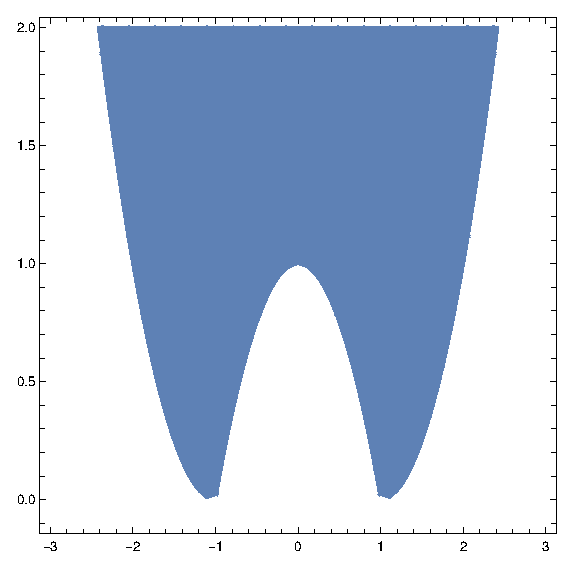
\includegraphics[width=\textwidth]{Chapter2/media/K1.eps}
         \caption{$K_1$}
        \label{fig.pwl.K1}
 \end{subfigure}
  \hfill
 \begin{subfigure}[b]{0.19\textwidth}
         \centering
         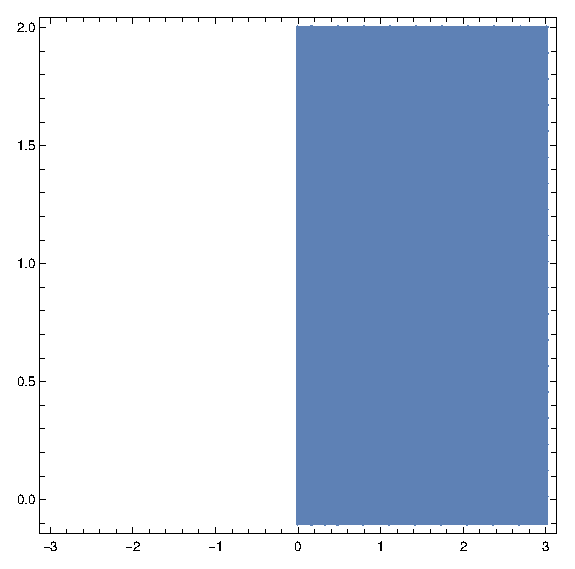
\includegraphics[width=\textwidth]{Chapter2/media/K2.eps}
         \caption{$K_2$}
        \label{fig.pwl.K2}
 \end{subfigure}
  \hfill
  \begin{subfigure}[b]{0.19\textwidth}
         \centering
         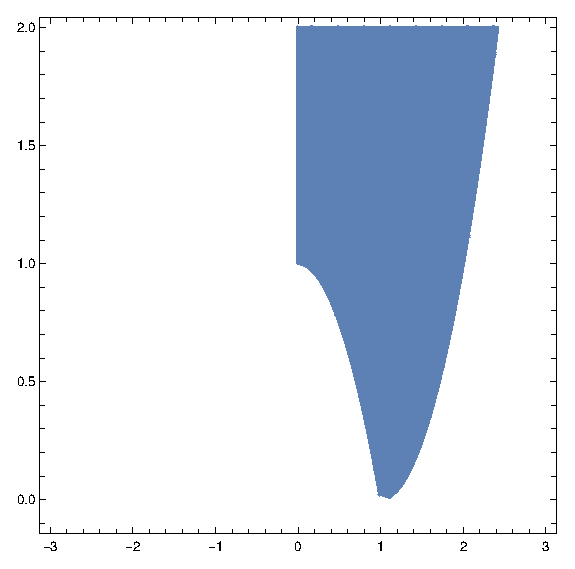
\includegraphics[width=\textwidth]{Chapter2/media/K.eps}
         \caption{$K$}
        \label{fig.pwl.K}
 \end{subfigure}
  \hfill
  \begin{subfigure}[b]{0.19\textwidth}
         \centering
         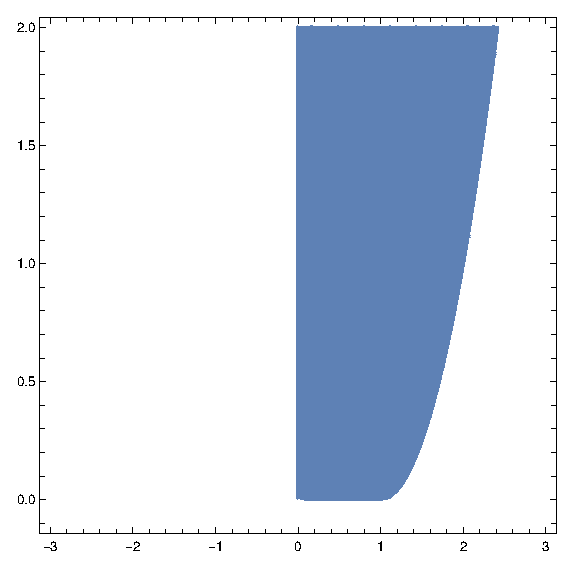
\includegraphics[width=\textwidth]{Chapter2/media/Khull.eps}
         \caption{$\conv(K_1) \cap K_2$}
        \label{fig.pwl.Khull}
 \end{subfigure}
  \hfill
   \begin{subfigure}[b]{0.19\textwidth}
         \centering
         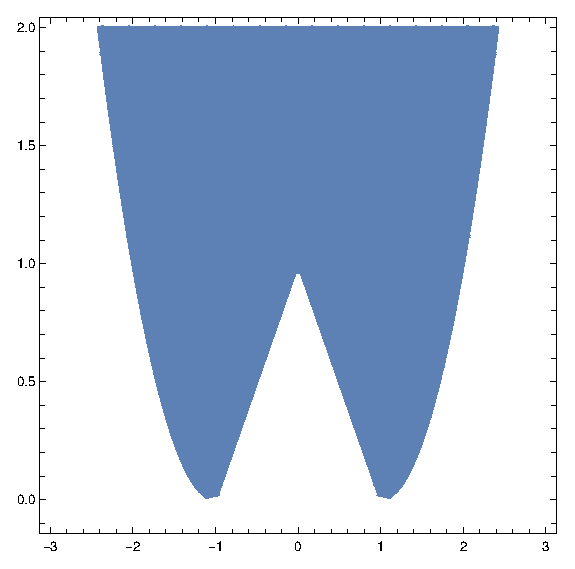
\includegraphics[width=\textwidth]{Chapter2/media/Kpwl.eps}
         \caption{$\bar{K}_1$}
        \label{fig.pwl.Kpwl}
 \end{subfigure}
  \caption{PWL approximation of nonconvex sets.}
  \label{fig.pwl}
\end{figure}




\section{Relaxation tightening via intersection cuts}
\label{sec.premic}
The cutting plane algorithm aims to construct a polyhedral outer approximation $P$ of the nonconvex set $\cS$, which is the feasible set of the MINLP problem $\min_{x \in \cS} c x$. Thereby, the polyhedron $P$ yields an LP relaxation of the MINLP problem.  Intersection cuts are a particular type of  valid inequalities that can tighten the polyhedral outer approximation.


The construction of intersection cuts \cite{conforti2014} requires two key ingredients: a simplicial cone containing  $\cS$, and an $\cS$-free set, which is defined as follows.

\begin{definition}
    \label{def.free}
    Given  a set $\cS \subsetneq \bR^p$, a closed set $\cC$ is (convex) $\cS$-free if $\cC$ is convex and $\inter(\cC) \cap \cS = \varnothing$.
    \end{definition}

Thinking reversely, $\cS$-free sets are convex regions whose  interiors have no element of $\cS$, so $\cS$-free sets can describe ``non-feasible'' regions of a MINLP problem.



\Cref{fig.sdef} shows an example of a $\cS$-free set, where we find  that  $\cC$ is a convex inner approximation of  $\cl(\cS^c)$.


Intersection cuts were initially devised in the continuous setting (the papers \cite{tuy64}, cited in \cite[Ch.~III]{horsttuy}, appeared before the classic paper \cite{balas1971intersection}), where they could approximate the hypograph $\cS$ of a convex function over a polytope.   There is a  unique  maximal  $\cS$-free set: the epigraph  of that convex function. Later, intersection cuts were used in the discrete setting \cite{balas1971intersection}, where $\cS$ is  a lattice. Several more families of lattice-free sets ({\eg}~splits, triangles, and spheres \cite{conforti2014,liberti2008spherical}) were described later.

We show how to construct $\cS$-free sets from a ``reverse'' representation of some nonconvex sets. We  look at  sets involving a particular type of nonconvex functions.

\begin{definition}
A function $f$ is said to be  difference-of-concave (DCC), if  there exists two concave functions $f_1,f_2$ such that $f=f_1 - f_2$.
\end{definition}

It is easy to show that the negative of a DCC function is also a DDC function, and thus any DC function is also a DCC function. A nonconvex set admits a \emph{DCC formulation}, if it is represented as the sublevel set of a DCC function. We call such a set \emph{a DCC set}.  The superlevel set of a DCC function is a sublevel set of another DDC function (the negative of that function), so one can reformulate the superlevel set into a DCC set.  For a  function $f$ and a point $\relx{x}$ in its domain, we denote the first-order approxiamtion $f(\relx{x}) + \nabla f(\relx{x})(x - \relx{x})$ of $f$ as $\lin{f}{\relx{x}}(x)$. The following  lemma gives a family of $\cS$-free sets for DCC sets via \emph{linearization method}.

\begin{lemma}[\cite{serrano2019}]\label{cor.dc2} 
Let $\cS := \{x \in \bR^p: f_1(x) - f_2(x) \le 0\}$, where  $f_1, f_2$ are concave functions over $\bR^p$. Then  for any $\relx{x} \in \bR^p$, $\cC := \{x \in \bR^p: f_1(x) - \lin{f_2}{\relx{x}}(x) \ge 0\}$ is $\cS$-free. Moreover, if $\relx{x} \in \bR^p \smallsetminus \cS$, $\relx{x} \in \inter(\cC)$.
\end{lemma}

To apply the above lemma, it suffices to reverse the inequality defining  $\cS$ and linearize its convex part. We refer to $\relx{x}$ as a \emph{linearization point} of $f_2$. Note that when the common domain  $\cG$ of $f_1$ and $f_2$ is not $\bR^p$,  $\cS$ should be restricted to the \emph{ground set} $\cG$.


\begin{figure}
 \centering
  \subfloat[$\cC$ as an $\cS$-free set.]{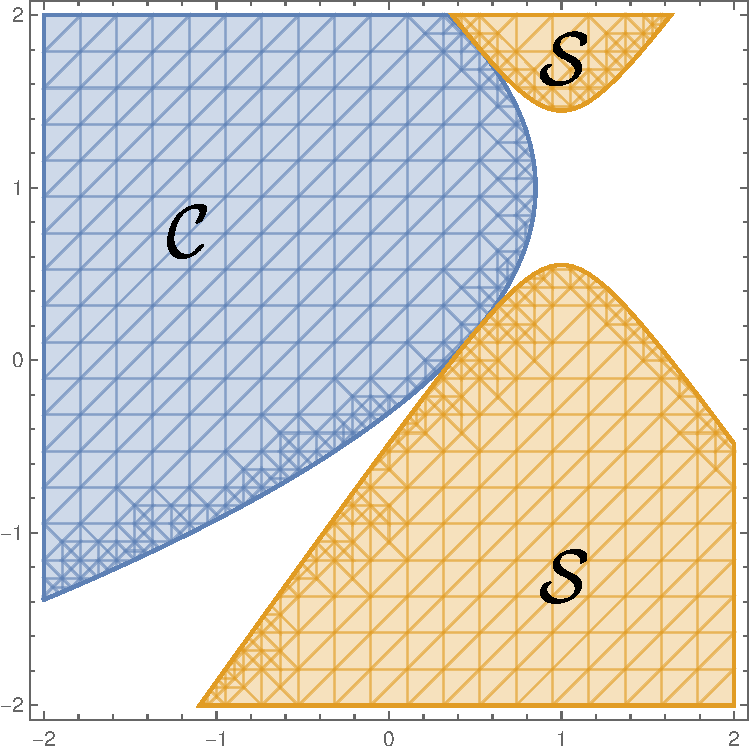
\includegraphics[width=0.3\textwidth]{Chapter2/media/sdef.pdf}}
  \hfill
  \subfloat[$\cC$ as an inner approximation of $\cl(\cS^c)$.]{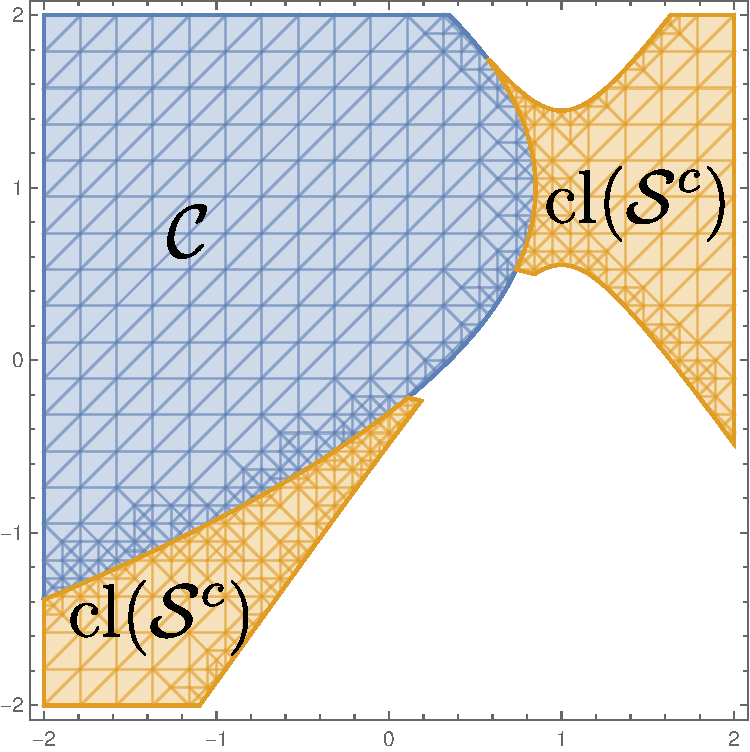
\includegraphics[width=0.3\textwidth]{Chapter2/media/sfreeinner.pdf}}
  \caption{An $\cS$-free set $\cC$.}
  \label{fig.sdef2}
\end{figure}
We show some examples in \Cref{fig.sdef2}.

Given an $\cS$-free set, the next step is to construct an intersection cut. The construction procedure requires additionally a translated polyhedral cone $\cR$  such that $\cS \subseteq \cR$ and the vertex $\relx{x}$  of $\cR$ is not in $\cS$. Let us suppose that $\cR$ admits a hyper-plane representation: $
     \{x \in \bR^p: B(x - \relx{x}) \le 0\}, $
where $B$ is a $p \times p$ invertible matrix. For all $j\in[p]$, let $r^j$ denote the $j$-th column of $-B^{-1}$, then $r^j$ turns out to be an extreme ray of $\cR$. Thereby, $\cR$ also admits a ray representation $
   \{x \in \bR^p:\exists \eta \in \bR^p_+ \textup{ }  x =\relx{x} +  \sum_{j =1}^{p} \eta_jr^j \}, $

    
For all $j \in [p]$, we define the \textit{step length} from $\relx{x}$ along ray $r_j$ to the boundary  $\bd(\cC)$ as
\begin{equation}
 \label{eq.iccoef}
   \eta_j^\ast := \max_{\eta_j \in [0,+\infty]}\{\eta_j: \relx{x} + \eta_j r^j \in \cC\}.
\end{equation}
Then, the intersection cut admits the form:
\begin{equation}
 \label{eq.ic}
     \sum_{j =1}^{p} \frac{1}{\eta_j^\ast} B_j (x - \relx{x}) \le -1,
 \end{equation}
where $B_j$ is the $j$-th row of $B$. When all step lengths are positive, the above linear inequality cuts off $\relx{x}$ from $\cS$.   The construction of an intersection cut is visualized in \Cref{fig.sdef}.

\begin{figure}
    \centering
     \subfloat[$\cC$ as an inner approximation of $\cl(\cS^c)$.]{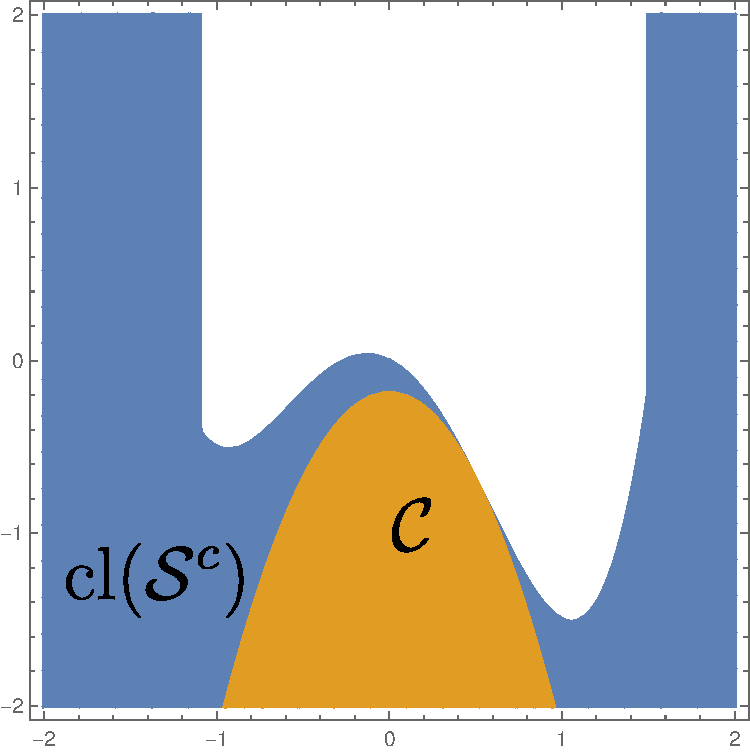
\includegraphics[width=0.3\textwidth]{Chapter2/media/s11.pdf}}
     \hfill
     \subfloat[$\cC$ as an $\cS$-free set.]{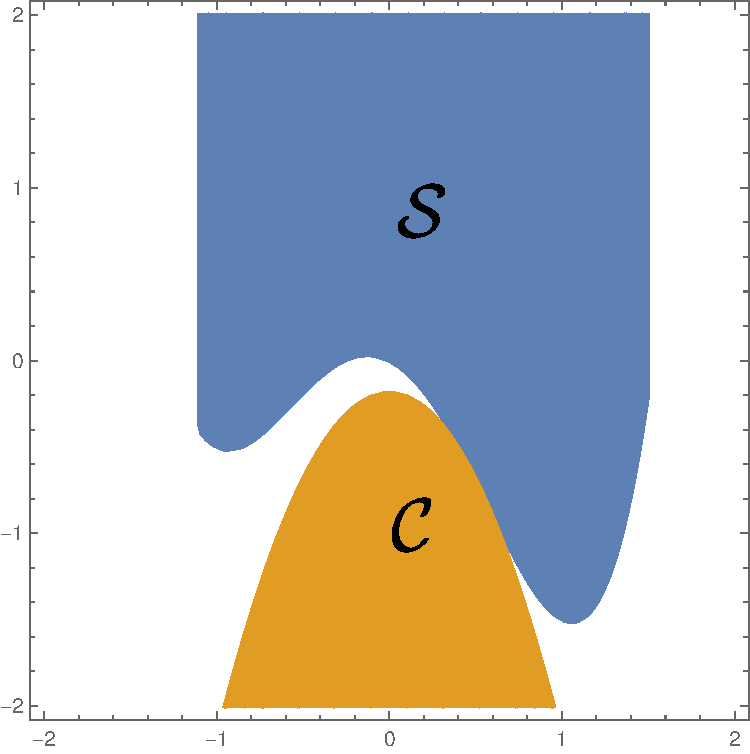
\includegraphics[width=0.3\textwidth]{Chapter2/media/s12.pdf}}
     \hfill
   \subfloat[Simplicial cone $\cR$ and the intersection cut.]{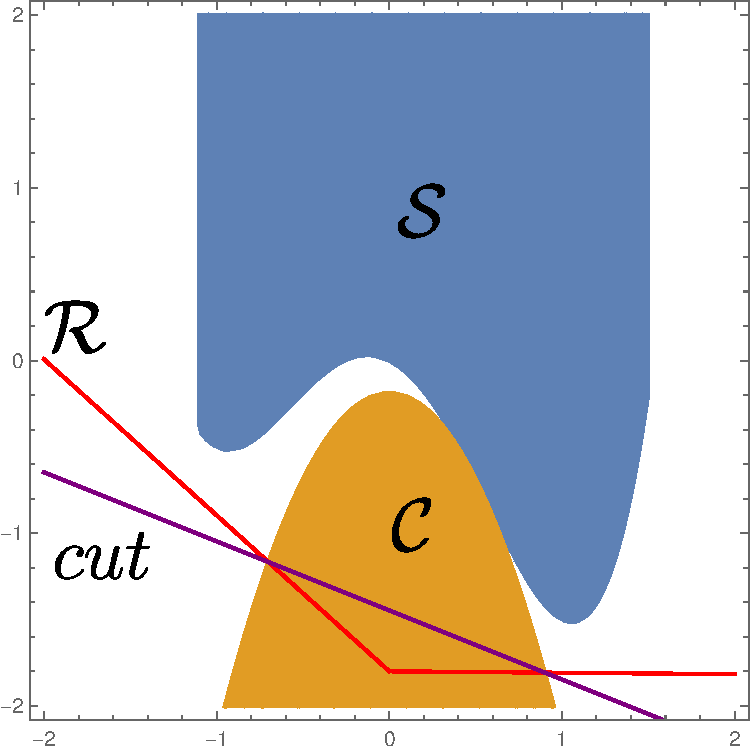
\includegraphics[width=0.3\textwidth]{Chapter2/media/s13.pdf}}
     \caption{An $\cS$-free set $\cC$, simplicial cone $\cR$, and intersection cut.}
     \label{fig.sdef}
   \end{figure}

In practice, we can obtain $\cS$, $\cR$, and $\relx{x}$  as follows. Assume that we have an LP relaxation $\min_{x \in \cP} c x$ of the MINLP problem, where $\cP$ is a polyhedral outer approximation of the feasible set. If the LP solution is not feasible to SP, as the LP relaxation usually comprises all linear constraints of the MINLP problem, then the solution must not satisfy some  nonlinear constraint.  Thus, we can set $\relx{x}$ to the LP solution and define $\cS$ by  the nonlinear constraint. Moreover,  we can extract $\cR$ from the basis of the LP defining $\relx{x}$. 


The main issue we address is therefore the construction of  (maximal) $\cS$-free sets.  The reason why we look for \emph{maximal} such sets is that, if
$\cC$ and $\cC^\ast$ are two $\cS$-free sets with $\cC \subseteq \cC^\ast$, then the intersection cut derived from $\cC^\ast$ dominates the intersection cut derived from $\cC$. Thereby, we give a formal definition of maximal $\cS$-free sets.

\begin{definition}
\label{def.max}
Given  a closed convex set $\cG \subseteq \bR^p$ such that $\cS \subsetneq \cG$, an  $\cS$-free set $\cC$ is (inclusion-wise) maximal in $\cG$,  if there is no other $\cS$-free set $\cC'$ such that $\cC \cap \cG \subsetneq \cC' \cap \cG $.
\end{definition}

\Cref{def.max} generalizes the conventional definition of  maximal $\cS$-free sets, and one can recover the conventional definition by setting $\cG = \bR^p$.  In some cases, it is difficult to study the maximality of $\cS$-free sets in $\bR^p$. \Cref{def.max} allows us to study intersections of $\cS$-free sets with the \emph{ground set}  $\cG$.  


\section{Conclusion}

In this section, we present a class of common relaxation methods. In the next chapter, we introduce some advanced theoretical results for relaxing structured sets. They yield new relaxation methods. In the rest of the thesis, we apply these methods to tackle applications that can be modelled as MINLP problems.
